\section{开关?电阻?(40pts)}
Nahida发现了一个古老的须弥电路图,如图\ref{switch} 所示,她想一会后意识到这个具有把开关当成电阻的功能。请你也来学习一下她的芝士吧!
\begin{figure}[htbp]
	\centering
	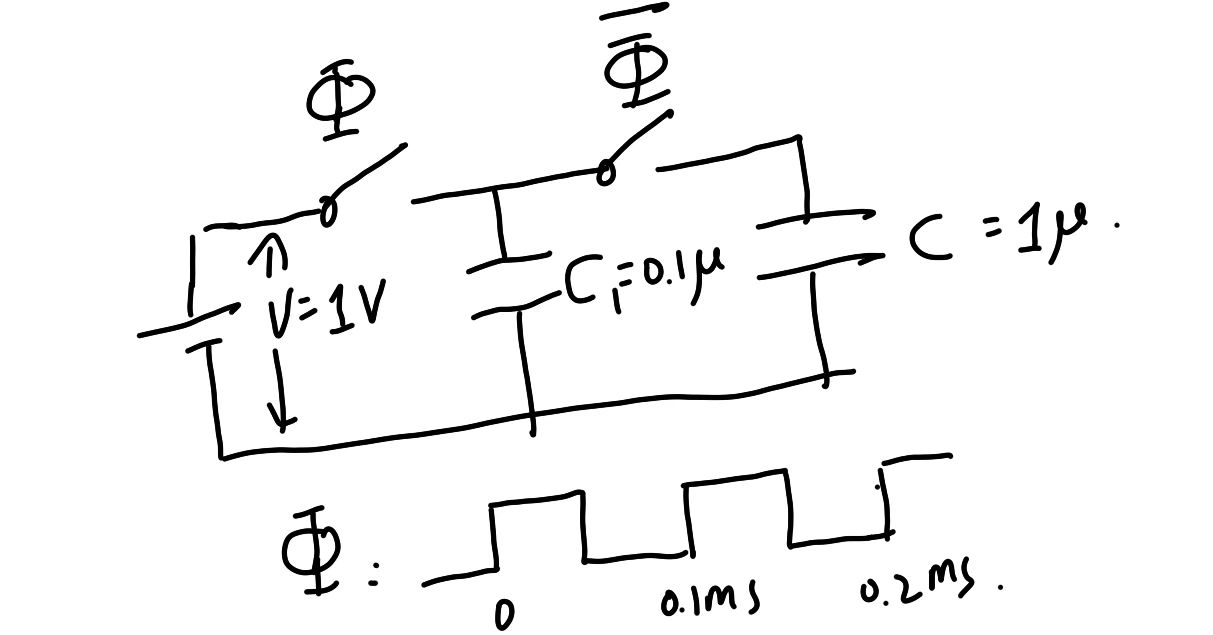
\includegraphics[width=0.5\textwidth]{switch}
	\caption{这是一个简单的电路图.}
	\label{switch}
\end{figure}
\begin{figure}[htbp]
	\centering
	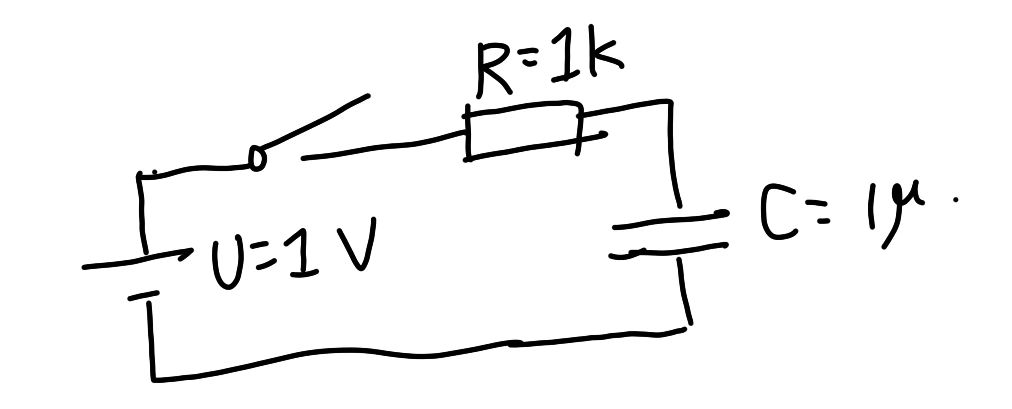
\includegraphics[width=0.5\textwidth]{RC}
	\caption{这真的是一个简单的电路图.}
	\label{RC}
\end{figure}
\begin{enumerate}
	\item 请求出图\ref{RC} 中的电容电压随时间的变化关系式\(V_c(t)\) (4pts)
	\item 请求出图\ref{switch} 中的电容电压随时间的变化关系式\(V_c'(t)\)。图示中有两个开关(cmos管)受到信号\(\Phi\)的控制,两个开关的信号恰好相反,只有当高电平的时候开关才会闭合。 硬件参数已经如图所示(24pts)
	\item 请给出若要把图示的开关完全等效为一个电阻\(R\)的条件,并且与原本的电容\(C\)无关。(12pts)
\end{enumerate}

\section*{Answer 6}
\begin{enumerate}
	\item 由电容充电公式可得:
	\begin{align*}
		V_c(t) &= V_0(1-e^{-t/RC}) 
	\end{align*}
	\item 不妨令\(T=0.1ms\),由于没有电阻,每一次都是速充。
	第一个T之后:
	\begin{align*}
		V_c'^{(1)} &= \frac{C_1}{C_1 + C} = \frac{1}{11} V
	\end{align*}
	在\(t=nT\),类推得到:
	\begin{align*}
		V_{c1}^{(n)}=V_c'^{(n)} &= \frac{C_1 +CV_{c1}^{(n-1)}}{C_1 + C}
	\end{align*}
	构造等比数列:
	\begin{align*}
		V_c^{(n)} - 1 = \frac{10}{11} (V_c^{(n-1)} - 1)
	\end{align*}
	\begin{align*}
		V_c^{(n)}=1- \left(\frac{10}{11}\right)^n
	\end{align*}
	加入取整函数得到:
	\begin{align*}
		V_c(t)=1- \left(\frac{10}{11}\right)^{[\frac{t}{T} + \frac{1}{2}]}
	\end{align*}
	\item 不难发现当\(T<<1,t>>T\)时,
	\begin{align*}
		V_c(t)=1- \left(\frac{10}{11}\right)^{[\frac{t}{T} + \frac{1}{2}]}\approx 1- e^{\ln(\frac{10}{11}) \frac{t}{T}}
	\end{align*}
	十分趋近于RC电路的充电公式了。如果在仔细观察一下的话,
	条件应该是:
	\begin{align*}
		\frac{1}{T}\ln(\frac{C_1+C}{C}) = \frac{1}{RC}
	\end{align*}
	当\(C_1<<C\)的时候,就有:
	\begin{align*}
		R \approx \frac{T}{C_1}
	\end{align*}
	此时电阻将于原本的电容大小无关了!这意味着我们可以用电容和开关转换成电阻,这在实际的数字电路中十分常见。


\end{enumerate}